This appendix contains information describing all of the data sets that were
used throughout the project for testing and profiling.

\begin{figure}[H]
    \centering
    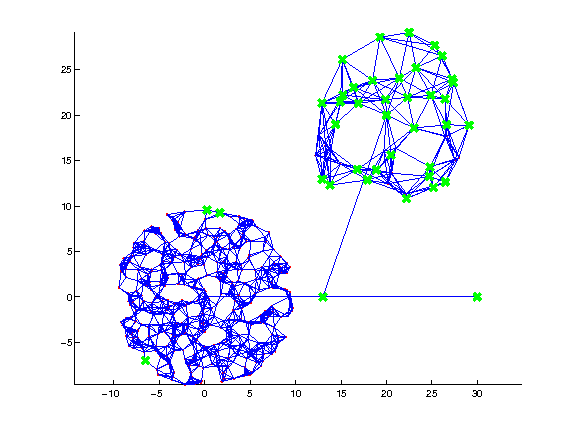
\includegraphics[width=0.5\textwidth]{./plots/pca/ball1}
    \caption{A PCA plot for the ball1 data set}
    \label{dataSets:ball1:pca}
\end{figure}

%%%%%%%%%%%%%%%%%%%%%%%%%%%%%%%%%%%%%%%%%%%%%%%%%
% DATASET 01: testoutrank
%%%%%%%%%%%%%%%%%%%%%%%%%%%%%%%%%%%%%%%%%%%%%%%%%
\section{testoutrank}
\label{datasets:testoutrank}
\begin{datasetDescription}{testoutrank}
    %\datasetProperty{Name}{}
    %\datasetProperty{Abstract}{}
    %\datasetProperty{Creators}{}
    %\datasetProperty{Donor}{}
    %\datasetProperty{Repository}{}
    %\datasetProperty{URL}{\url{}}
    %\datasetProperty{Date}{\formatdate{}{}{}}
    %
    \datasetProperty{Number of instances ($M$)}{441}
    \datasetProperty{Number of attributes ($N$)}{2}
    %\datasetProperty{Data set characteristics}{}
    %\datasetProperty{Attribute characteristics}{}
    %\datasetProperty{Attribute information}{
    %    \begin{itemize}
    %        \item 
    %    \end{itemize}
    %}
    %
    %\datasetProperty{Data set information}{
    %}
\end{datasetDescription}

%%%%%%%%%%%%%%%%%%%%%%%%%%%%%%%%%%%%%%%%%%%%%%%%%
% DATASET 02: ball1
%%%%%%%%%%%%%%%%%%%%%%%%%%%%%%%%%%%%%%%%%%%%%%%%%
\section{ball1}
\label{datasets:ball1}
\begin{datasetDescription}{ball1}
    %\datasetProperty{Name}{}
    %\datasetProperty{Abstract}{}
    %\datasetProperty{Creators}{}
    %\datasetProperty{Donor}{}
    %\datasetProperty{Repository}{}
    %\datasetProperty{URL}{\url{}}
    %\datasetProperty{Date}{\formatdate{}{}{}}
    %
    \datasetProperty{Number of instances ($M$)}{552}
    \datasetProperty{Number of attributes ($N$)}{2}
    %\datasetProperty{Data set characteristics}{}
    %\datasetProperty{Attribute characteristics}{}
    %\datasetProperty{Attribute information}{
    %    \begin{itemize}
    %        \item 
    %    \end{itemize}
    %}
    %
    %\datasetProperty{Data set information}{
    %}
\end{datasetDescription}

%%%%%%%%%%%%%%%%%%%%%%%%%%%%%%%%%%%%%%%%%%%%%%%%%
% DATASET 03: testCD
%%%%%%%%%%%%%%%%%%%%%%%%%%%%%%%%%%%%%%%%%%%%%%%%%
\section{testCD}
\label{datasets:testCD}
\begin{datasetDescription}{testCD}
    %\datasetProperty{Name}{}
    %\datasetProperty{Abstract}{}
    %\datasetProperty{Creators}{}
    %\datasetProperty{Donor}{}
    %\datasetProperty{Repository}{}
    %\datasetProperty{URL}{\url{}}
    %\datasetProperty{Date}{\formatdate{}{}{}}
    %
    \datasetProperty{Number of instances ($M$)}{640}
    \datasetProperty{Number of attributes ($N$)}{2}
    %\datasetProperty{Data set characteristics}{}
    %\datasetProperty{Attribute characteristics}{}
    %\datasetProperty{Attribute information}{
    %    \begin{itemize}
    %        \item 
    %    \end{itemize}
    %}
    %
    %\datasetProperty{Data set information}{
    %}
\end{datasetDescription}

%%%%%%%%%%%%%%%%%%%%%%%%%%%%%%%%%%%%%%%%%%%%%%%%%
% DATASET 04: runningex1k
%%%%%%%%%%%%%%%%%%%%%%%%%%%%%%%%%%%%%%%%%%%%%%%%%
\section{runningex1k}
\label{datasets:runningex1k}
\begin{datasetDescription}{runningex1k}
    %\datasetProperty{Name}{}
    %\datasetProperty{Abstract}{}
    %\datasetProperty{Creators}{}
    %\datasetProperty{Donor}{}
    %\datasetProperty{Repository}{}
    %\datasetProperty{URL}{\url{}}
    %\datasetProperty{Date}{\formatdate{}{}{}}
    %
    \datasetProperty{Number of instances ($M$)}{1000}
    \datasetProperty{Number of attributes ($N$)}{2}
    %\datasetProperty{Data set characteristics}{}
    %\datasetProperty{Attribute characteristics}{}
    %\datasetProperty{Attribute information}{
    %    \begin{itemize}
    %        \item 
    %    \end{itemize}
    %}
    %
    %\datasetProperty{Data set information}{
    %}
\end{datasetDescription}

%%%%%%%%%%%%%%%%%%%%%%%%%%%%%%%%%%%%%%%%%%%%%%%%%
% DATASET 05: testCDST2
%%%%%%%%%%%%%%%%%%%%%%%%%%%%%%%%%%%%%%%%%%%%%%%%%
\section{testCDST2}
\label{sec:datasets:testCDST2}
\begin{datasetDescription}{testCDST2}
    %\datasetProperty{Name}{}
    %\datasetProperty{Abstract}{}
    %\datasetProperty{Creators}{}
    %\datasetProperty{Donor}{}
    %\datasetProperty{Repository}{}
    %\datasetProperty{URL}{\url{}}
    %\datasetProperty{Date}{\formatdate{}{}{}}
    %
    \datasetProperty{Number of instances ($M$)}{2000}
    \datasetProperty{Number of attributes ($N$)}{2}
    %\datasetProperty{Data set characteristics}{}
    %\datasetProperty{Attribute characteristics}{}
    %\datasetProperty{Attribute information}{
    %    \begin{itemize}
    %        \item 
    %    \end{itemize}
    %}
    %
    %\datasetProperty{Data set information}{
    %}
\end{datasetDescription}

%%%%%%%%%%%%%%%%%%%%%%%%%%%%%%%%%%%%%%%%%%%%%%%%%
% DATASET 06: testCDST3
%%%%%%%%%%%%%%%%%%%%%%%%%%%%%%%%%%%%%%%%%%%%%%%%%
\section{testCDST3}
\label{sec:datasets:testCDST3}
\begin{datasetDescription}{testCDST3}
    %\datasetProperty{Name}{}
    %\datasetProperty{Abstract}{}
    %\datasetProperty{Creators}{}
    %\datasetProperty{Donor}{}
    %\datasetProperty{Repository}{}
    %\datasetProperty{URL}{\url{}}
    %\datasetProperty{Date}{\formatdate{}{}{}}
    %
    \datasetProperty{Number of instances ($M$)}{2000}
    \datasetProperty{Number of attributes ($N$)}{2}
    %\datasetProperty{Data set characteristics}{}
    %\datasetProperty{Attribute characteristics}{}
    %\datasetProperty{Attribute information}{
    %    \begin{itemize}
    %        \item 
    %    \end{itemize}
    %}
    %
    %\datasetProperty{Data set information}{
    %}
\end{datasetDescription}

%%%%%%%%%%%%%%%%%%%%%%%%%%%%%%%%%%%%%%%%%%%%%%%%%
% DATASET 07: testCDST
%%%%%%%%%%%%%%%%%%%%%%%%%%%%%%%%%%%%%%%%%%%%%%%%%
\section{testCDST}
\label{sec:datasets:testCDST}
\begin{datasetDescription}{testCDST}
    %\datasetProperty{Name}{}
    %\datasetProperty{Abstract}{}
    %\datasetProperty{Creators}{}
    %\datasetProperty{Donor}{}
    %\datasetProperty{Repository}{}
    %\datasetProperty{URL}{\url{}}
    %\datasetProperty{Date}{\formatdate{}{}{}}
    %
    \datasetProperty{Number of instances ($M$)}{2000}
    \datasetProperty{Number of attributes ($N$)}{2}
    %\datasetProperty{Data set characteristics}{}
    %\datasetProperty{Attribute characteristics}{}
    %\datasetProperty{Attribute information}{
    %    \begin{itemize}
    %        \item 
    %    \end{itemize}
    %}
    %
    %\datasetProperty{Data set information}{
    %}
\end{datasetDescription}

%%%%%%%%%%%%%%%%%%%%%%%%%%%%%%%%%%%%%%%%%%%%%%%%%
% DATASET 08: runningex10k
%%%%%%%%%%%%%%%%%%%%%%%%%%%%%%%%%%%%%%%%%%%%%%%%%
\section{runningex10k}
\label{sec:datasets:runningex10k}
\begin{datasetDescription}{runningex10k}
    %\datasetProperty{Name}{}
    %\datasetProperty{Abstract}{}
    %\datasetProperty{Creators}{}
    %\datasetProperty{Donor}{}
    %\datasetProperty{Repository}{}
    %\datasetProperty{URL}{\url{}}
    %\datasetProperty{Date}{\formatdate{}{}{}}
    %
    \datasetProperty{Number of instances ($M$)}{10000}
    \datasetProperty{Number of attributes ($N$)}{2}
    %\datasetProperty{Data set characteristics}{}
    %\datasetProperty{Attribute characteristics}{}
    %\datasetProperty{Attribute information}{
    %    \begin{itemize}
    %        \item 
    %    \end{itemize}
    %}
    %
    %\datasetProperty{Data set information}{
    %}
\end{datasetDescription}

%%%%%%%%%%%%%%%%%%%%%%%%%%%%%%%%%%%%%%%%%%%%%%%%%
% DATASET 09: runningex20k
%%%%%%%%%%%%%%%%%%%%%%%%%%%%%%%%%%%%%%%%%%%%%%%%%
\section{runningex20k}
\label{sec:datasets:runningex20k}
\begin{datasetDescription}{runningex20k}
    %\datasetProperty{Name}{}
    %\datasetProperty{Abstract}{}
    %\datasetProperty{Creators}{}
    %\datasetProperty{Donor}{}
    %\datasetProperty{Repository}{}
    %\datasetProperty{URL}{\url{}}
    %\datasetProperty{Date}{\formatdate{}{}{}}
    %
    \datasetProperty{Number of instances ($M$)}{20000}
    \datasetProperty{Number of attributes ($N$)}{2}
    %\datasetProperty{Data set characteristics}{}
    %\datasetProperty{Attribute characteristics}{}
    %\datasetProperty{Attribute information}{
    %    \begin{itemize}
    %        \item 
    %    \end{itemize}
    %}
    %
    %\datasetProperty{Data set information}{
    %}
\end{datasetDescription}

%%%%%%%%%%%%%%%%%%%%%%%%%%%%%%%%%%%%%%%%%%%%%%%%%
% DATASET 10: segmentation
%%%%%%%%%%%%%%%%%%%%%%%%%%%%%%%%%%%%%%%%%%%%%%%%%
\section{segmentation}
\label{sec:datasets:segmentation}
\begin{datasetDescription}{segmentation}
    \datasetProperty{Name}{Image Segmentation Data}
    \datasetProperty{Creators}{Vision Group, University of Massachusetts}
    \datasetProperty{Donor}{Carla Brodley [Vision Group]}
    \datasetProperty{Repository}{School of Science and Technology, University of
        New England}
    \datasetProperty{URL}{\url{http://turing.une.edu.au/~comp513/Data/segment-test.arff}}
    \datasetProperty{Date}{\formatdate{1}{11}{1990}}
    %
    \datasetProperty{Number of instances ($M$)}{2100}
    \datasetProperty{Number of attributes ($N$)}{19 + 1 class attribute}
    \datasetProperty{Attribute information}{
        \begin{itemize}
            \item[region-centroid-col] The column of the center pixel of the
                region.
            \item[region-centroid-row] The row of the center pixel of the
                region.
            \item[region-pixel-count] The number of pixels in a region
                (\ensuremath{=9}).
            \item[short-line-density-5] The results of a line extraction
                algorithm that counts how many lines of length 5 (any
                orientation) with low contrast, less than or equal to 5, go
                through the region.
            \item[short-line-density-2] Same as \lstinline+short-line-density-5+
                but counts lines of high contrast, greater than 5.
            \item[vedge-mean] Measure the contrast of horizontally adjacent
                pixels in the region. There are 6, the mean and standard
                deviation are given.  This attribute is used as a vertical edge
                detector.
            \item[vegde-sd] See \lstinline+verge-mean+.
            \item[hedge-mean] Measures the contrast of vertically adjacent
                pixels. Used for horizontal line detection..
            \item[hedge-sd] See \lstinline+hedge-mean+.
            \item[intensity-mean] The average over the region of
                \ensuremath{\left(R+G+B\right)/3}
            \item[rawred-mean] The average over the region of the
                \ensuremath{R} value.
            \item[rawblue-mean] The average over the region of the
                \ensuremath{B} value.
            \item[rawgreen-mean] The average over the region of the
                \ensuremath{G} value.
            \item[exred-mean] Measure the excess red:
                \ensuremath{\left(2R-\left(G+B\right)\right)}.
            \item[exblue-mean] Measure the excess blue:
                \ensuremath{\left(2B-\left(G+R\right)\right)}.
            \item[exgreen-mean] Measure the excess green:
                \ensuremath{\left(2G-\left(R+B\right)\right)}.
            \item[value-mean] 3-d nonlinear transformation of RGB.
            \item[saturation-mean] See \lstinline+value_mean+.
            \item[hue-mean] See \lstinline+value_mean+.
        \end{itemize}
    }
    %
    \datasetProperty{Data set information}{
    The instances were drawn randomly from a database of 7 outdoor images. The
    images were unsegmented to create a classification for every pixel. Each
    instance is a $3 \times 3$ region.
    }
\end{datasetDescription}

%%%%%%%%%%%%%%%%%%%%%%%%%%%%%%%%%%%%%%%%%%%%%%%%%
% DATASET 11: spam_train
%%%%%%%%%%%%%%%%%%%%%%%%%%%%%%%%%%%%%%%%%%%%%%%%%
\section{spam\_train}
\label{sec:datasets:spam_train}
\begin{datasetDescription}{spam_train}
    %\datasetProperty{Name}{}
    %\datasetProperty{Abstract}{}
    %\datasetProperty{Creators}{}
    %\datasetProperty{Donor}{}
    %\datasetProperty{Repository}{}
    %\datasetProperty{URL}{\url{}}
    %\datasetProperty{Date}{\formatdate{}{}{}}
    %
    \datasetProperty{Number of instances ($M$)}{4501}
    \datasetProperty{Number of attributes ($N$)}{58}
    %\datasetProperty{Data set characteristics}{}
    %\datasetProperty{Attribute characteristics}{}
    %\datasetProperty{Attribute information}{
    %    \begin{itemize}
    %        \item 
    %    \end{itemize}
    %}
    %
    %\datasetProperty{Data set information}{
    %}
\end{datasetDescription}

%%%%%%%%%%%%%%%%%%%%%%%%%%%%%%%%%%%%%%%%%%%%%%%%%
% DATASET 12: runningex30k
%%%%%%%%%%%%%%%%%%%%%%%%%%%%%%%%%%%%%%%%%%%%%%%%%
\section{runningex30k}
\label{sec:datasets:runningex30k}
\begin{datasetDescription}{runningex30k}
    %\datasetProperty{Name}{}
    %\datasetProperty{Abstract}{}
    %\datasetProperty{Creators}{}
    %\datasetProperty{Donor}{}
    %\datasetProperty{Repository}{}
    %\datasetProperty{URL}{\url{}}
    %\datasetProperty{Date}{\formatdate{}{}{}}
    %
    \datasetProperty{Number of instances ($M$)}{30000}
    \datasetProperty{Number of attributes ($N$)}{2}
    %\datasetProperty{Data set characteristics}{}
    %\datasetProperty{Attribute characteristics}{}
    %\datasetProperty{Attribute information}{
    %    \begin{itemize}
    %        \item 
    %    \end{itemize}
    %}
    %
    %\datasetProperty{Data set information}{
    %}
\end{datasetDescription}

%%%%%%%%%%%%%%%%%%%%%%%%%%%%%%%%%%%%%%%%%%%%%%%%%
% DATASET 13: pendigits
%%%%%%%%%%%%%%%%%%%%%%%%%%%%%%%%%%%%%%%%%%%%%%%%%
\section{pendigits}
\label{sec:datasets:pendigits}
\begin{datasetDescription}{pendigits}
    \datasetProperty{Name}{Pen-Based Recognition of Handwritten Digits Data Set}
    \datasetProperty{Abstract}{Digit database of 250 samples from 44 writers.}
    \datasetProperty{Creators}{
        E. Alpaydin, Fevzi. Alimoglu
        [Department of Computer Engineering, Bogazici University]
    }
    \datasetProperty{Repository}{UCI Machine Learning Repository}
    \datasetProperty{URL}{\url{http://archive.ics.uci.edu/ml/datasets/Pen-Based+Recognition+of+Handwritten+Digits}}
    \datasetProperty{Date}{\formatdate{1}{7}{1998}}
    %
    \datasetProperty{Number of instances ($M$)}{10992}
    \datasetProperty{Number of attributes ($N$)}{16 + 1 class attribute}
    \datasetProperty{Data set characteristics}{Multivariate}
    \datasetProperty{Attribute characteristics}{Integer}
    \datasetProperty{Attribute information}{
        \begin{itemize}
            \item All input attributes are integers in the range
                $\left[0,100\right]$.
            \item The last attribute is the class code $\left[0,9\right]$.
        \end{itemize}
    }
    %
    \datasetProperty{Data set information \cite{Frank:2010}}{
        A digit database obtained by collecting 250 samples from 44 writers. The
        samples written by 30 writers were used for training, cross-validation
        and writer dependent testing, and the digits written by the other 14
        were used for writer independent testing.
        \newline
        The data was obtained using a WACOM PL-100V pressure sensitive tablet
        with an integrated LCD display and a cordless stylus. The input and
        display areas are located in the same place. The tablet sends $x$ and
        $y$ tablet coordinates and pressure level values of the pen at fixed
        time intervals (sampling rate) of 100 miliseconds.
        \newline
        The writers are asked to write 250 digits in random order inside boxes
        of 500 by 500 tablet pixel resolution. In the study, only the
        $\left(x,y\right)$ coordinate information --- the stylus pressure level
        values were ignored. Normalization was applied to make the
        representation invariant to translations and scale distortions. The raw
        data that was capture from the tablet consisted of integer values
        $\left[0,500\right]$ (tablet input box resolution). The new coordinates
        are such that the coordinate which has the maximum range varies between
        0 and 100. Usually $x$ stays in this range, since most characters are
        taller than they are wide.
        \newline
        In order to represent digits as constant length feature vectors, the
        data was resampled using simple linear interpolation between pairs of
        points. The resampled digits are represented as a sequence of $T$ points
        $\left(x_t,y_t\right)_{t=1}^T$, regularly spaced in arc length, as
        opposed to the input sequence, which is regularly spaced in time.
        \newline
        So, the input vector size is $2 \times T$, twice the number of points
        resampled. The value $T=8$ gave the best trade-off between accuracy and
        complexity.
    }
\end{datasetDescription}

%%%%%%%%%%%%%%%%%%%%%%%%%%%%%%%%%%%%%%%%%%%%%%%%%
% DATASET 14: runningex40k
%%%%%%%%%%%%%%%%%%%%%%%%%%%%%%%%%%%%%%%%%%%%%%%%%
\section{runningex40k}
\label{sec:datasets:runningex40k}
\begin{datasetDescription}{runningex40k}
    %\datasetProperty{Name}{}
    %\datasetProperty{Abstract}{}
    %\datasetProperty{Creators}{}
    %\datasetProperty{Donor}{}
    %\datasetProperty{Repository}{}
    %\datasetProperty{URL}{\url{}}
    %\datasetProperty{Date}{\formatdate{}{}{}}
    %
    \datasetProperty{Number of instances ($M$)}{40000}
    \datasetProperty{Number of attributes ($N$)}{2}
    %\datasetProperty{Data set characteristics}{}
    %\datasetProperty{Attribute characteristics}{}
    %\datasetProperty{Attribute information}{
    %    \begin{itemize}
    %        \item 
    %    \end{itemize}
    %}
    %
    %\datasetProperty{Data set information}{
    %}
\end{datasetDescription}

%%%%%%%%%%%%%%%%%%%%%%%%%%%%%%%%%%%%%%%%%%%%%%%%%
% DATASET 15: runningex50k
%%%%%%%%%%%%%%%%%%%%%%%%%%%%%%%%%%%%%%%%%%%%%%%%%
\section{runningex50k}
\label{sec:datasets:runningex50k}
\begin{datasetDescription}{runningex50k}
    %\datasetProperty{Name}{}
    %\datasetProperty{Abstract}{}
    %\datasetProperty{Creators}{}
    %\datasetProperty{Donor}{}
    %\datasetProperty{Repository}{}
    %\datasetProperty{URL}{\url{}}
    %\datasetProperty{Date}{\formatdate{}{}{}}
    %
    \datasetProperty{Number of instances ($M$)}{50000}
    \datasetProperty{Number of attributes ($N$)}{2}
    %\datasetProperty{Data set characteristics}{}
    %\datasetProperty{Attribute characteristics}{}
    %\datasetProperty{Attribute information}{
    %    \begin{itemize}
    %        \item 
    %    \end{itemize}
    %}
    %
    %\datasetProperty{Data set information}{
    %}
\end{datasetDescription}

%%%%%%%%%%%%%%%%%%%%%%%%%%%%%%%%%%%%%%%%%%%%%%%%%
% DATASET 16: spam
%%%%%%%%%%%%%%%%%%%%%%%%%%%%%%%%%%%%%%%%%%%%%%%%%
\section{spam}
\label{sec:datasets:spam}
\nocite{Frank:2010}
\begin{datasetDescription}{spam}
    \datasetProperty{Name}{Spambase data set}
    \datasetProperty{Abstract}{Classifying email as spam or non-spam.}
    \datasetProperty{Creators}{
        Mark Hopkins, Erik Reeber, George Forman, Jaap Suermondt
        [Hewlett-Packard Labs]
    }
    \datasetProperty{Donor}{George Forman}
    \datasetProperty{Repository}{UCI Machine Learning Repository}
    \datasetProperty{URL}{\url{http://archive.ics.uci.edu/ml/datasets/Spambase}}
    \datasetProperty{Date}{\formatdate{1}{7}{1999}}
    %
    \datasetProperty{Number of instances ($M$)}{4601}
    \datasetProperty{Number of attributes ($N$)}{57 + 1 class attribute}
    \datasetProperty{Data set characteristics}{Multivariate}
    \datasetProperty{Attribute characteristics}{Integer, Real}
    \datasetProperty{Attribute information}{
        Most of the attributes indicate whether a particular word or character
        was frequently occurring in the email. The run-length attributes
        $\left[55,57\right]$ measure the length of sequences of consecutive
        capital letters.
        \newline
        \begin{itemize}
            \item 48 continuous real \ensuremath{\left[0,100\right]} attributes
                of type \lstinline+word_freq_WORD+, equal to the percentage of
                words in the email that match \lstinline+WORD+. A
                \lstinline+word+ in this case is any string of alphanumeric
                characters bounded by non-alphanumeric characters or
                end-of-string.
            \item 6 continuous real \ensuremath{\left[0,100\right]} attributes
                of type \lstinline+char_freq_CHAR+, equal to the percentage of
                characters in the email that match \lstinline+CHAR+.
            \item 1 continuous real \ensuremath{\left[1,\ldots\right]} attribute
                of type \lstinline+capital_run_length_average+, equal to the
                average length of uninterrupted sequences of capital letters.
            \item 1 continuous integer \ensuremath{\left[1,\ldots\right]}
                attribute of type \lstinline+capital_run_length_longest+, equal
                to the length of longest uninterrupted sequence of capital
                letters.
            \item 1 continuous integer \ensuremath{\left[1,\ldots\right]}
                attribute of type \lstinline+capital_run_length_total+, equal to
                the sum of length of uninterrupted sequences of capital letters.
            \item 1 nominal \ensuremath{\left\{0,1\right\}} class attribute of
                type \lstinline+spam+, which denotes whether the email was
                considered spam (\ensuremath{1}) or not (\ensuremath{0}), i.e.\ 
                unsolicited commercial e-mail).
        \end{itemize}
    }
    %
    \datasetProperty{Data set information \cite{Frank:2010}}{
        The collection of \lstinline+spam+ emails came from a postmaster, as
        well as from individuals who had filed spam. The collection of
        \lstinline+non-spam+ emails came from filed work and personal emails.
    }
\end{datasetDescription}

%%%%%%%%%%%%%%%%%%%%%%%%%%%%%%%%%%%%%%%%%%%%%%%%%
% DATASET 17: letter-recognition
%%%%%%%%%%%%%%%%%%%%%%%%%%%%%%%%%%%%%%%%%%%%%%%%%
\section{letter-recognition}
\label{sec:datasets:letter-recognition}
\nocite{Frank:2010}
\begin{datasetDescription}{letter-recognition}
    \datasetProperty{Name}{Letter Recognition Data Set}
    \datasetProperty{Abstract}{Database of character image features; trying to
        identify the letter.}
    \datasetProperty{Creator}{David J. Slate [Odesta Corporation]}
    \datasetProperty{Donor}{David J. Slate [Odesta Corporation]}
    \datasetProperty{Repository}{UCI Machine Learning Repository}
    \datasetProperty{URL}{\url{http://archive.ics.uci.edu/ml/datasets/Letter+Recognition}}
    \datasetProperty{Date}{\formatdate{1}{1}{1991}}
    %
    \datasetProperty{Number of instances ($M$)}{20000}
    \datasetProperty{Number of attributes ($N$)}{16 + 1 class attribute}
    \datasetProperty{Data set characteristics}{Multivariate}
    \datasetProperty{Attribute characteristics}{Integer}
    \datasetProperty{Attribute information}{
        \begin{description}
            \item[lettr] Capital letter.
            \item[x-box] Horizontal position of box.
            \item[y-box] Vertical position of box.
            \item[width] Width of box.
            \item[high]  Height of box.
            \item[onpix] Total number on pixels.
            \item[x-bar] Mean \ensuremath{x} of on pixels in box.
            \item[y-bar] Mean \ensuremath{y} of on pixels in box.
            \item[x2bar] Mean \ensuremath{x} variance.
            \item[y2bar] Mean \ensuremath{y} variance.
            \item[xybar] Mean \ensuremath{\left(x,y\right)} correlation.
            \item[x2ybr] Mean of \ensuremath{x^{2}y}.
            \item[xy2br] Mean of \ensuremath{xy^{2}}.
            \item[x-ege] Mean edge count left to right.
            \item[xegvy] Correlation of \ensuremath{x-ege} with \ensuremath{y}.
            \item[y-ege] Mean edge count bottom to top.
            \item[yegvx] Correlation of \ensuremath{y-ege} with \ensuremath{x}.
        \end{description}
    }
    %
    \datasetProperty{Data set information \cite{Frank:2010}}{
        The objective was to identify each of a large number of black-and-white
        rectangular pixel displays as one of the 26 capital letters in the
        English alphabet. The character images were based on 20 different fonts
        and each letter within these 20 fonts was randomly distorted to produce
        a file of 20000 unique stimuli. Each stimulus was converted into 16
        primitive numerical attributes (statistical moments and edge counts)
        which were then scaled to fit into a range of integer values
        $\left[0,15\right]$.
    }
\end{datasetDescription}

%%%%%%%%%%%%%%%%%%%%%%%%%%%%%%%%%%%%%%%%%%%%%%%%%
% DATASET 18: mesh_network
%%%%%%%%%%%%%%%%%%%%%%%%%%%%%%%%%%%%%%%%%%%%%%%%%
\section{mesh\_network}
\label{sec:datasets:mesh_network}
\begin{datasetDescription}{mesh_network}
    \datasetProperty{Name}{NICTA Wireless Mesh Network}
    %\datasetProperty{Abstract}{}
    %\datasetProperty{Creators}{}
    %\datasetProperty{Donor}{}
    %\datasetProperty{Repository}{}
    %\datasetProperty{URL}{\url{}}
    %\datasetProperty{Date}{\formatdate{}{}{}}
    %
    \datasetProperty{Number of instances ($M$)}{1193}
    \datasetProperty{Number of attributes ($N$)}{392}
    %\datasetProperty{Data set characteristics}{}
    %\datasetProperty{Attribute characteristics}{}
    %\datasetProperty{Attribute information}{
    %    \begin{itemize}
    %        \item 
    %    \end{itemize}
    %}
    %
    \datasetProperty{Data set information}{
        The NICTA wireless mesh network has seven nodes deployed at the
        University of Sydney. It used a traffic generator to simulate the
        traffic on the network. Packets were aggregated into one minute time bins
        and the data were collected in 24 hours. There were 391 OD flows and
        1270 time bins. Four anomalies were introduced to the network where
        three of them were DOS attacks and one was a ping flood.
    }
\end{datasetDescription}

%%%%%%%%%%%%%%%%%%%%%%%%%%%%%%%%%%%%%%%%%%%%%%%%%
% DATASET 19: magicgamma
%%%%%%%%%%%%%%%%%%%%%%%%%%%%%%%%%%%%%%%%%%%%%%%%%
\section{magicgamma}
\label{sec:datasets:magicgamma}
\nocite{Frank:2010}
\begin{datasetDescription}{magicgamma}
    \datasetProperty{Name}{MAGIC Gamma Telescope Data Set}
    \datasetProperty{Abstract}{Data are MC generated to simulate registration of
        high energy gamma particles in an atmospheric Cherenkov telescope.}
    \datasetProperty{Original owner}{
        R. K. Bock
        [Major Atmospheric Gamma Imaging Cherenkov Telescope project (MAGIC)]
    }
    \datasetProperty{Donor}{
        P. Savicky
        [Institute of Computer Science, AS of CR]
    }
    \datasetProperty{Repository}{UCI Machine Learning Repository}
    \datasetProperty{URL}{\url{http://archive.ics.uci.edu/ml/datasets/MAGIC+Gamma+Telescope}}
    \datasetProperty{Date}{\formatdate{1}{5}{2007}}
    %
    \datasetProperty{Number of instances ($M$)}{19020}
    \datasetProperty{Number of attributes ($N$)}{11}
    \datasetProperty{Data set characteristics}{Multivariate}
    \datasetProperty{Attribute characteristics}{Real}
    \datasetProperty{Attribute information}{
        \begin{description}
            \item [fLength] Major axis of ellipse (in millimetres).
            \item [fWidth] Minor axis of ellipse (in millimetres).
            \item [fSize] Common logarithm of sum of content of all pixels.
            \item [fConc] Ratio of sum of two highest pixels over
                \lstinline+fSize+.
            \item [fConc1] Ratio of highest pixel over \lstinline+fSize+.
            \item [fAsym] Distance from highest pixel to center, projected onto
                major axis (in millimetres).
            \item [fM3Long] Third root of third moment along major axis (in
                millimetres).
            \item [fM3Trans] Third root of third moment along minor axis (in
                millimetres).
            \item [fAlpha] Angle of major axis with vector to origin (in
                degrees).
            \item [fDist] Distance from origin to center of ellipse (in
                millimetres).
            \item [class] Either gamma (signal) or hadron (background).
        \end{description}
    }
    %
    \datasetProperty{Data set information \cite{Frank:2010}}{
        The data are MC generated to simulate registration of high energy gamma
        particles in a ground-based atmospheric Cherenkov gamma telescope using
        the imaging technique. Cherenkov gamma telescope observes high energy
        gamma rays, taking advantage of the radiation emitted by charged
        particles produced inside the electromagnetic showers initiated by the
        gammas, and developing in the atmosphere. This Cherenkov radiation (of
        visible to UV wavelengths) leaks through the atmosphere and gets
        recorded in the detector, allowing reconstruction of the shower
        parameters. The available information consists of pulses left by the
        incoming Cherenkov photons on the photomultiplier tubes, arranged in a
        plane, the camera. Depending on the energy of the primary gamma, a total
        of few hundreds to some 10000 Cherenkov photons get collected, in
        patterns (called the shower image), allowing to discriminate
        statistically those caused by primary gammas (signal) from the images of
        hadronic showers initiated by cosmic rays in the upper atmosphere
        (background).
    }
\end{datasetDescription}

%%%%%%%%%%%%%%%%%%%%%%%%%%%%%%%%%%%%%%%%%%%%%%%%%
% DATASET 20: musk
%%%%%%%%%%%%%%%%%%%%%%%%%%%%%%%%%%%%%%%%%%%%%%%%%
\section{musk}
\label{sec:datasets:musk}
\nocite{Frank:2010}
\begin{datasetDescription}{musk}
    \datasetProperty{Name}{Musk (Version 2) Data Set}
    \datasetProperty{Abstract}{The goal is to learn to predict whether new
        molecules will be musks or non-musks}
    \datasetProperty{Creators}{
        David Chapman, Ajay Jain
        [AI Group at Arris Pharmaceutical Corporation]
    }
    \datasetProperty{Donor}{Tom Dietterich}
    \datasetProperty{Repository}{UCI Machine Learning Repository}
    \datasetProperty{URL}{\url{http://http://archive.ics.uci.edu/ml/datasets/Musk+(Version+2)}}
    \datasetProperty{Date}{\formatdate{12}{9}{1994}}
    %
    \datasetProperty{Number of instances ($M$)}{6598}
    \datasetProperty{Number of attributes ($N$)}{167 + 1 class attribute (note
        that one attribute has been discarded)}
    \datasetProperty{Data set characteristics}{Multivariate}
    \datasetProperty{Attribute characteristics}{Integer}
    \datasetProperty{Attribute information}{
        \begin{description}
            \item[molecule\_name] Symbolic name of each molecule. Musks have
                names such as \lstinline+MUSK-188+. Non-musks have names such as
                \lstinline+NON-MUSK-jp13+.
            \item[conformation\_name] Symbolic name of each conformation. These
                have the format \lstinline|MOL_ISO+CONF|, where \lstinline+MOL+
                is the molecule number, \lstinline+ISO+ is the stereoisomer
                number (usually 1), and \lstinline+CONF+ is the conformation
                number.
            \item[\ensuremath{\left\{f_1,\ldots,f_162\right\}}] These are
                ``distance features'' along rays. The distances are measured in
                hundredths of Angstroms. The distances may be negative or
                positive, since they are actually measured relative to an origin
                placed along each ray. The origin was defined by a ``consensus
                musk'' surface that is no longer used. Hence, any experiments
                with the data should treat these feature values as lying on an
                arbitrary continuous scale. In particular, the algorithm should
                not make any use of the zero point or the sign of each feature
                value.
            \item[\ensuremath{f_163} (OXY-DIS)] This is the distance of the
                oxygen atom in the molecule to a designated point in 3-space.
            \item[\ensuremath{f_164} (OXY-X)] \ensuremath{X}-displacement from
                the designated point.
            \item[\ensuremath{f_165} (OXY-Y)] \ensuremath{Y}-displacement from
                the designated point.
            \item[\ensuremath{f_166} (OXY-Z)] \ensuremath{Z}-displacement from
                the designated point.
            \item[class] \ensuremath{0} if non-musk; \ensuremath{1} if musk.
        \end{description}
    }
    %
    \datasetProperty{Data set information \cite{Frank:2010}}{
        This data set describes a set of 102 molecules of which 39 are judged by
        human experts to be musks and the remaining 63 molecules are judged to
        be non-musks. The goal was to learn to predict whether new molecules
        were musks or non-musks. However, the 166 features that describe these
        molecules depend upon the exact shape, or conformation, of the molecule.
        Because bonds can rotate, a single molecule can adopt many different
        shapes. To generate this data set, all the low-energy conformations of
        the molecules were generated to produce 6598 conformations. Then, a
        feature vector was extracted that describes each conformation.
    }
\end{datasetDescription}

%%%%%%%%%%%%%%%%%%%%%%%%%%%%%%%%%%%%%%%%%%%%%%%%%
% DATASET 21: connect4
%%%%%%%%%%%%%%%%%%%%%%%%%%%%%%%%%%%%%%%%%%%%%%%%%
\section{connect4}
\label{sec:datasets:connect4}
\nocite{Frank:2010}
\begin{datasetDescription}{connect4}
    \datasetProperty{Name}{Connect-4 Data Set}
    \datasetProperty{Abstract}{Contains connect-4 positions.}
    \datasetProperty{Original owner}{John Tromp}
    \datasetProperty{Donor}{John Tromp}
    \datasetProperty{Repository}{UCI Machine Learning Repository}
    \datasetProperty{URL}{\url{http://archive.ics.uci.edu/ml/datasets/Connect-4}}
    \datasetProperty{Date}{\formatdate{4}{2}{1995}}
    %
    \datasetProperty{Number of instances ($M$)}{67557}
    \datasetProperty{Number of attributes ($N$)}{42 + 1 class attribute}
    \datasetProperty{Data set characteristics}{Multivariate, Spatial}
    \datasetProperty{Attribute characteristics}{Categorical}
    \datasetProperty{Attribute information}{
        The columns of the board are labelled $\left\{a,b,c,d,e,f,g\right\}$
        (from left to right). The rows of the board are labelled
        $\left\{1,2,3,4,5,6\right\}$ (from bottom to top). There are 42 fields
        representing the board positions $\left(row,column\right)$. $x$ is the
        first player and $o$ is the second. $b$ represents a blank square. The
        \lstinline+outcome+ class is the game theoretical value for the first
        player, $\left\{win,draw,loss\right\}$.
    }
    %
    \datasetProperty{Data set information \cite{Frank:2010}}{
        This database contains all legal 8-ply positions in the game of
        connect-4 in which neither player has won yet, and in which the next
        move is not forced.
    }
\end{datasetDescription}
